\documentclass{standalone}
\usepackage{tikz}
\usetikzlibrary{patterns, positioning}


\begin{document}
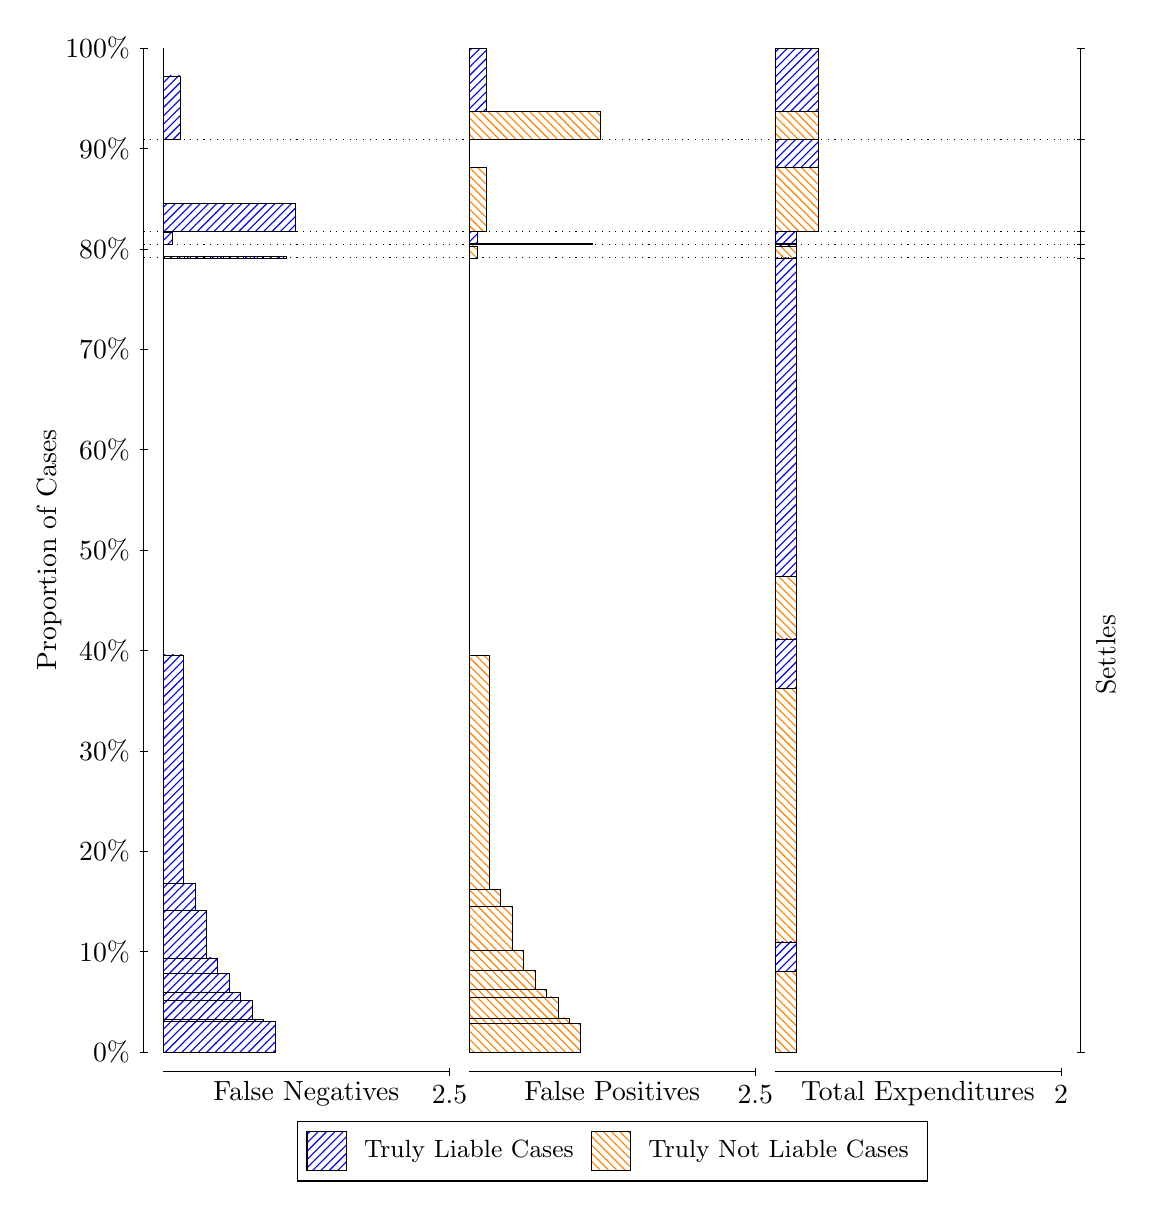
\begin{tikzpicture}
\draw[black, very thin] (1.5,1.75) -- (1.5,14.5);
\node[rotate=90, text=black, anchor=center] at (0.3, 8.125) {Proportion of Cases};
\draw[black, very thin] (1.45,1.75) -- (1.55,1.75);
\node[text=black, anchor=east] at (1.45, 1.75) {0\%};
\draw[black, very thin] (1.45,3.025) -- (1.55,3.025);
\node[text=black, anchor=east] at (1.45, 3.025) {10\%};
\draw[black, very thin] (1.45,4.3) -- (1.55,4.3);
\node[text=black, anchor=east] at (1.45, 4.3) {20\%};
\draw[black, very thin] (1.45,5.575) -- (1.55,5.575);
\node[text=black, anchor=east] at (1.45, 5.575) {30\%};
\draw[black, very thin] (1.45,6.85) -- (1.55,6.85);
\node[text=black, anchor=east] at (1.45, 6.85) {40\%};
\draw[black, very thin] (1.45,8.125) -- (1.55,8.125);
\node[text=black, anchor=east] at (1.45, 8.125) {50\%};
\draw[black, very thin] (1.45,9.4) -- (1.55,9.4);
\node[text=black, anchor=east] at (1.45, 9.4) {60\%};
\draw[black, very thin] (1.45,10.675) -- (1.55,10.675);
\node[text=black, anchor=east] at (1.45, 10.675) {70\%};
\draw[black, very thin] (1.45,11.95) -- (1.55,11.95);
\node[text=black, anchor=east] at (1.45, 11.95) {80\%};
\draw[black, very thin] (1.45,13.225) -- (1.55,13.225);
\node[text=black, anchor=east] at (1.45, 13.225) {90\%};
\draw[black, very thin] (1.45,14.5) -- (1.55,14.5);
\node[text=black, anchor=east] at (1.45, 14.5) {100\%};

\draw[black, very thin] (13.4,1.75) -- (13.4,14.5);
\draw[black, very thin] (13.35,1.75) -- (13.45,1.75);
\node[anchor=west] at (13.35, 1.75) {};
\draw[black, very thin] (13.35,11.835) -- (13.45,11.835);
\node[anchor=west] at (13.35, 11.835) {};
\draw[black, very thin] (13.35,12.005) -- (13.45,12.005);
\node[anchor=west] at (13.35, 12.005) {};
\draw[black, very thin] (13.35,12.175) -- (13.45,12.175);
\node[anchor=west] at (13.35, 12.175) {};
\draw[black, very thin] (13.35,13.339) -- (13.45,13.339);
\node[anchor=west] at (13.35, 13.339) {};
\draw[black, very thin] (13.35,14.5) -- (13.45,14.5);
\node[anchor=west] at (13.35, 14.5) {};

\draw[black, very thin, pattern color=blue, pattern=north east lines] (1.75,1.75) rectangle (3.167,2.1342);
\draw[black, very thin, pattern color=blue, pattern=north east lines] (1.75,2.1342) rectangle (3.0217,2.1632);
\draw[black, very thin, pattern color=blue, pattern=north east lines] (1.75,2.1632) rectangle (2.8763,2.4014);
\draw[black, very thin, pattern color=blue, pattern=north east lines] (1.75,2.4014) rectangle (2.731,2.5079);
\draw[black, very thin, pattern color=blue, pattern=north east lines] (1.75,2.5079) rectangle (2.5857,2.7506);
\draw[black, very thin, pattern color=blue, pattern=north east lines] (1.75,2.7506) rectangle (2.4403,2.9443);
\draw[black, very thin, pattern color=blue, pattern=north east lines] (1.75,2.9443) rectangle (2.295,3.5458);
\draw[black, very thin, pattern color=blue, pattern=north east lines] (1.75,3.5458) rectangle (2.1497,3.8893);
\draw[black, very thin, pattern color=blue, pattern=north east lines] (1.75,3.8893) rectangle (2.0043,6.794);
\draw[black, very thin, pattern color=orange, pattern=north west lines] (1.75,6.794) rectangle (1.75,11.835);
\draw[black, very thin, pattern color=blue, pattern=north east lines] (1.75,11.835) rectangle (3.3123,11.852);
\draw[black, very thin, pattern color=orange, pattern=north west lines] (1.75,11.852) rectangle (1.75,12.005);
\draw[black, very thin, pattern color=blue, pattern=north east lines] (1.75,12.005) rectangle (1.859,12.158);
\draw[black, very thin, pattern color=orange, pattern=north west lines] (1.75,12.158) rectangle (1.75,12.175);
\draw[black, very thin, pattern color=blue, pattern=north east lines] (1.75,12.175) rectangle (3.4213,12.529);
\draw[black, very thin, pattern color=orange, pattern=north west lines] (1.75,12.529) rectangle (1.75,13.339);
\draw[black, very thin, pattern color=blue, pattern=north east lines] (1.75,13.339) rectangle (1.968,14.146);
\draw[black, very thin, pattern color=orange, pattern=north west lines] (1.75,14.146) rectangle (1.75,14.5);
\draw[black, very thin, pattern color=orange, pattern=north west lines] (5.6333,1.75) rectangle (7.0503,2.1167);
\draw[black, very thin, pattern color=orange, pattern=north west lines] (5.6333,2.1167) rectangle (6.905,2.1831);
\draw[black, very thin, pattern color=orange, pattern=north west lines] (5.6333,2.1831) rectangle (6.7597,2.4486);
\draw[black, very thin, pattern color=orange, pattern=north west lines] (5.6333,2.4486) rectangle (6.6143,2.544);
\draw[black, very thin, pattern color=orange, pattern=north west lines] (5.6333,2.544) rectangle (6.469,2.7867);
\draw[black, very thin, pattern color=orange, pattern=north west lines] (5.6333,2.7867) rectangle (6.3237,3.0358);
\draw[black, very thin, pattern color=orange, pattern=north west lines] (5.6333,3.0358) rectangle (6.1783,3.5993);
\draw[black, very thin, pattern color=orange, pattern=north west lines] (5.6333,3.5993) rectangle (6.033,3.8117);
\draw[black, very thin, pattern color=orange, pattern=north west lines] (5.6333,3.8117) rectangle (5.8877,6.791);
\draw[black, very thin, pattern color=blue, pattern=north east lines] (5.6333,6.791) rectangle (5.6333,11.835);
\draw[black, very thin, pattern color=orange, pattern=north west lines] (5.6333,11.835) rectangle (5.7423,11.988);
\draw[black, very thin, pattern color=blue, pattern=north east lines] (5.6333,11.988) rectangle (5.6333,12.005);
\draw[black, very thin, pattern color=orange, pattern=north west lines] (5.6333,12.005) rectangle (7.1957,12.021);
\draw[black, very thin, pattern color=blue, pattern=north east lines] (5.6333,12.021) rectangle (5.7423,12.175);
\draw[black, very thin, pattern color=orange, pattern=north west lines] (5.6333,12.175) rectangle (5.8513,12.985);
\draw[black, very thin, pattern color=blue, pattern=north east lines] (5.6333,12.985) rectangle (5.6333,13.339);
\draw[black, very thin, pattern color=orange, pattern=north west lines] (5.6333,13.339) rectangle (7.3047,13.693);
\draw[black, very thin, pattern color=blue, pattern=north east lines] (5.6333,13.693) rectangle (5.8513,14.5);
\draw[black, very thin, pattern color=orange, pattern=north west lines] (9.5167,1.75) rectangle (9.7892,2.775);
\draw[black, very thin, pattern color=blue, pattern=north east lines] (9.5167,2.775) rectangle (9.7892,3.1487);
\draw[black, very thin, pattern color=orange, pattern=north west lines] (9.5167,3.1487) rectangle (9.7892,6.3706);
\draw[black, very thin, pattern color=blue, pattern=north east lines] (9.5167,6.3706) rectangle (9.7892,6.9975);
\draw[black, very thin, pattern color=orange, pattern=north west lines] (9.5167,6.9975) rectangle (9.7892,7.7916);
\draw[black, very thin, pattern color=blue, pattern=north east lines] (9.5167,7.7916) rectangle (9.7892,11.835);
\draw[black, very thin, pattern color=orange, pattern=north west lines] (9.5167,11.835) rectangle (9.7892,11.988);
\draw[black, very thin, pattern color=blue, pattern=north east lines] (9.5167,11.988) rectangle (9.7892,12.005);
\draw[black, very thin, pattern color=orange, pattern=north west lines] (9.5167,12.005) rectangle (9.7892,12.021);
\draw[black, very thin, pattern color=blue, pattern=north east lines] (9.5167,12.021) rectangle (9.7892,12.175);
\draw[black, very thin, pattern color=orange, pattern=north west lines] (9.5167,12.175) rectangle (10.062,12.985);
\draw[black, very thin, pattern color=blue, pattern=north east lines] (9.5167,12.985) rectangle (10.062,13.339);
\draw[black, very thin, pattern color=orange, pattern=north west lines] (9.5167,13.339) rectangle (10.062,13.693);
\draw[black, very thin, pattern color=blue, pattern=north east lines] (9.5167,13.693) rectangle (10.062,14.5);
\draw[black, dotted] (1.5,11.835) -- (13.4,11.835);
\draw[black, dotted] (1.5,12.005) -- (13.4,12.005);
\draw[black, dotted] (1.5,12.175) -- (13.4,12.175);
\draw[black, dotted] (1.5,13.339) -- (13.4,13.339);
\draw[black, very thin] (1.75,1.5) -- (5.3833,1.5);
\node[text=black, anchor=north] at (3.5667, 1.5) {False Negatives};
\draw[black, very thin] (5.3833,1.45) -- (5.3833,1.55);
\node[text=black, anchor=north] at (5.3833, 1.45) {2.5};

\draw[black, very thin] (5.6333,1.5) -- (9.2667,1.5);
\node[text=black, anchor=north] at (7.45, 1.5) {False Positives};
\draw[black, very thin] (9.2667,1.45) -- (9.2667,1.55);
\node[text=black, anchor=north] at (9.2667, 1.45) {2.5};

\draw[black, very thin] (9.5167,1.5) -- (13.15,1.5);
\node[text=black, anchor=north] at (11.333, 1.5) {Total Expenditures};
\draw[black, very thin] (13.15,1.45) -- (13.15,1.55);
\node[text=black, anchor=north] at (13.15, 1.45) {2};

\node[text=black, centered, rotate=90] at (13.72, 6.7925) {Settles};





\draw (7.449999999999999,1.5) node[draw=none] (baseCoordinate) {};
\begin{scope}[align=center]
        \matrix[scale=0.5, draw=black, below=0.5cm of baseCoordinate, nodes={draw}, column sep=0.1cm]{
            \node[rectangle, draw, minimum width=0.5cm, minimum height=0.5cm, pattern color=blue, pattern=north east lines] {}; &
            \node[draw=none, font=\small, text=black] (B) {Truly Liable Cases}; &
            \node[rectangle, draw, minimum width=0.5cm, minimum height=0.5cm, pattern color=orange, pattern=north west lines] {}; &
            \node[draw=none, font=\small, text=black] (B) {Truly Not Liable Cases}; \\
            };
\end{scope}

\end{tikzpicture}
\end{document}